%*----------- SLIDE -------------------------------------------------------------
\begin{frame}[t]{Methods to image analysis}
    \begin{figure}
        \centering
        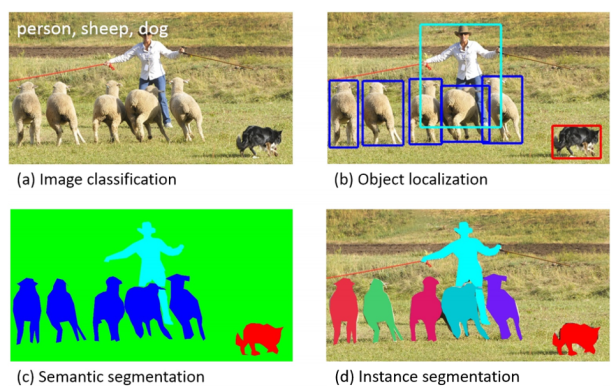
\includegraphics[width=0.55\textwidth]{methods}
        \caption{Methods to image analysis. \cite{lin2014microsoft}}
    \end{figure}
\end{frame}
%-

%*----------- SLIDE -------------------------------------------------------------
\begin{frame}[c]{Semantic Segmentation applied in video}
    \centering
    \includemedia[
        width=0.7\linewidth,
        totalheight=0.39375\linewidth,
        activate=pageopen,
        passcontext, 
        addresource=./Media/pictures/seg_video.mp4,
        flashvars={
        source=./Media/pictures/seg_video.mp4
        &autoPlay=true
        &Loop=false}
        ]{\fbox{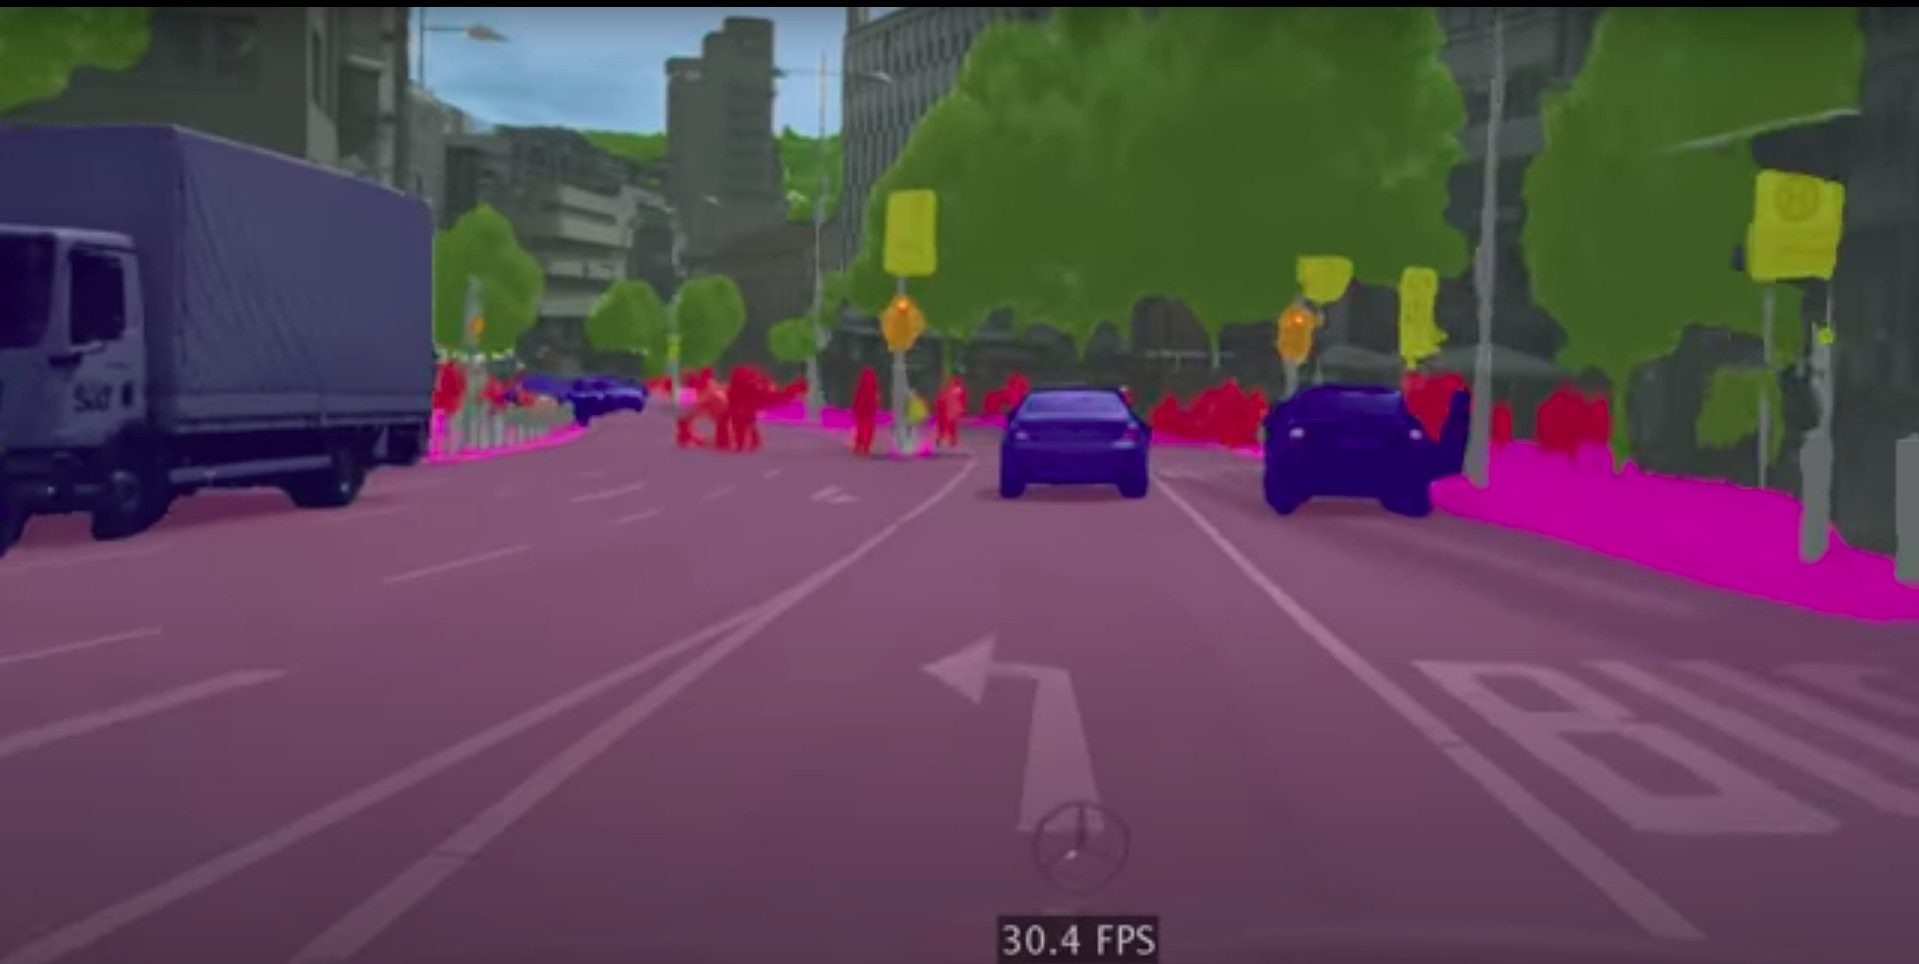
\includegraphics{seg_video}}}{VPlayer.swf}

    Semantic Segmentation \cite{semseg}
\end{frame}
%-

\begin{frame}[t]{Semantic Segmentation}
    \begin{columns}[c]
        \column{.05\textwidth}
        \column{.6\textwidth}
            \newline
            \newline
                Use \textbf{ImageNet} pre-trained networks
            \newline
            \newline
                Smaller dataset, even \textbf{worse} for RGB-D and 3D datasets
            \newline
            \newline
                Use \textbf{synthetic datasets} extracted from commercial video games
           
        \column{.35\textwidth}
        \newline
        \newline
        \newline
        \newline
        \begin{flushright}
            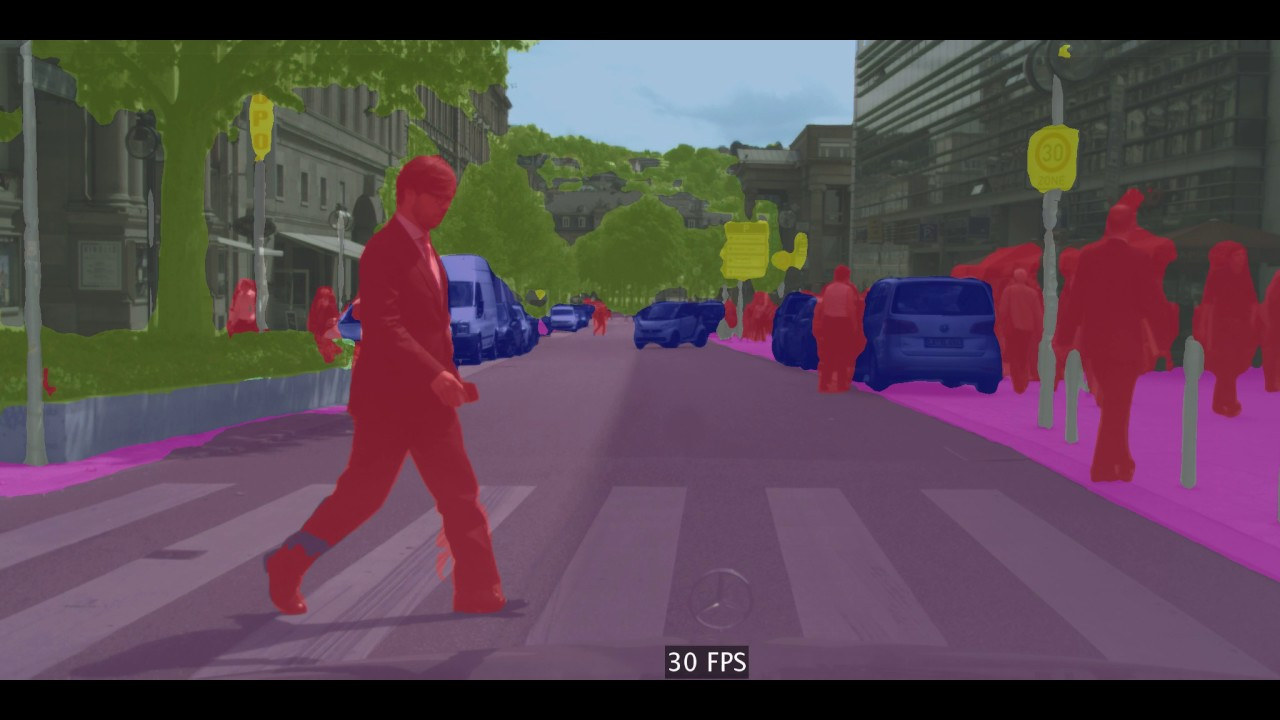
\includegraphics[width=1\textwidth]{semantic}
        \end{flushright} 
    \end{columns}
    
\end{frame}